\newpage
\section{Anhang}

%\begin{figure}[h]
%    \centering
%    \includegraphics[width=0.7\textwidth]{latex/images/messwerte.jpeg}
%    \caption{Die Messwerte der Interferenzmaximaanzahl}
%    \label{img:mess1}
%\end{figure}
%  
\begin{figure}[h]
    \centering
    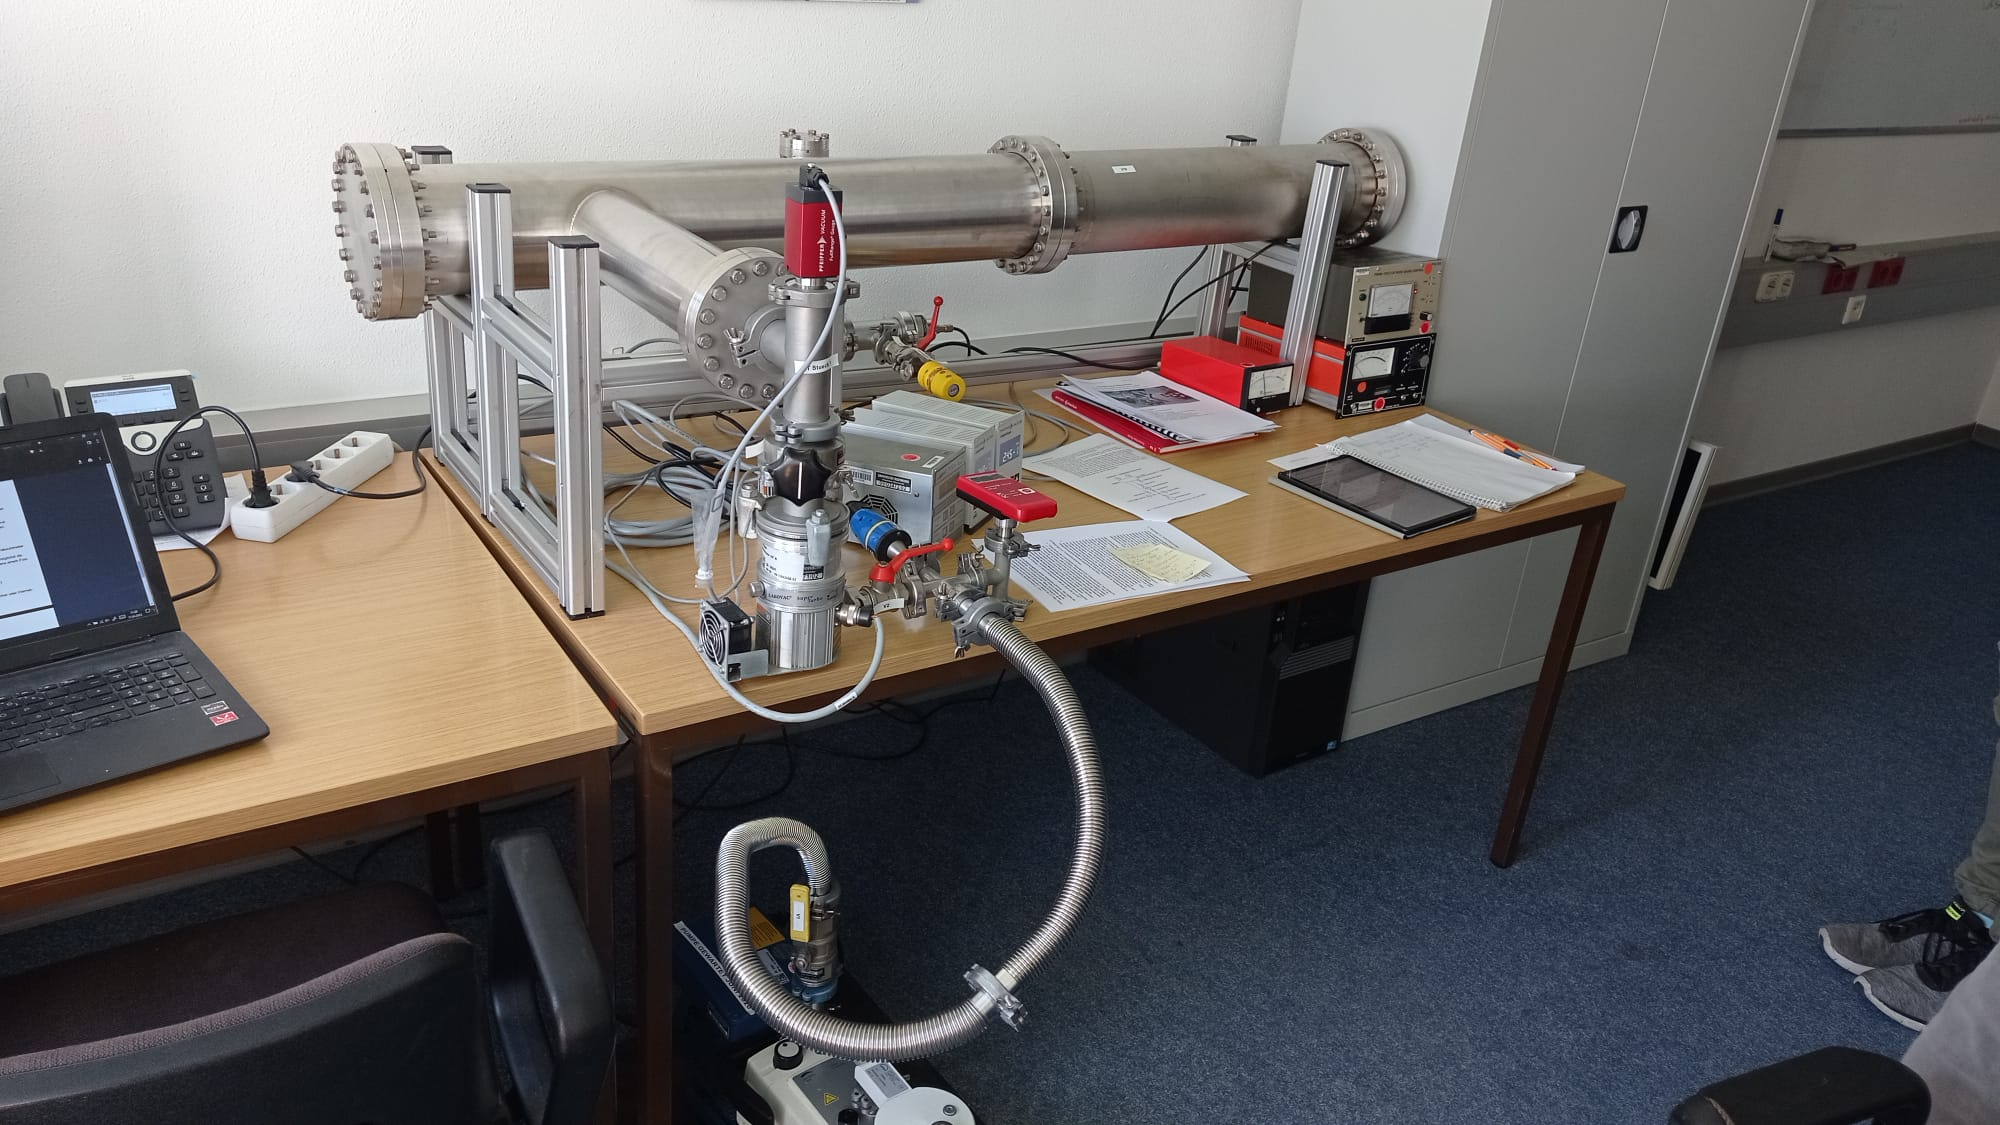
\includegraphics[width=0.7\textwidth]{latex/images/Aufbau.jpeg}
    \caption{Der Versuchsaufbau des Michelson-Interferometers}
\end{figure}


\subsection{Messwerte}

\begin{table}[H]
\small
\centering
\begin{tabular}{S [table-format=2.3] S [table-format=2.3] S [table-format=2.3] c }
    \toprule
    \multicolumn{1}{p{3.2cm}}{\centering$\text{Druck Messreihe 1 } $\\$ \text{in }\si{\milli\bar}$} &
    \multicolumn{1}{p{3.2cm}}{\centering$\text{Druck Messreihe 2 } $\\$ \text{in }\si{\milli\bar}$} &
    \multicolumn{1}{p{3.2cm}}{\centering$\text{Druck Messreihe 3 } $\\$ \text{in }\si{\milli\bar}$} &
    \multicolumn{1}{p{3.2cm}}{\centering$\text{Druck gemittelt } $\\$ \text{in }\si{\milli\bar}$} \\
    \midrule
    0.101 & 0.103 & 0.1   & 0.1013 \pm 0.0012 \\
    0.251 & 0.258 & 0.252 & 0.2537 \pm 0.0031 \\
    0.378 & 0.386 & 0.375 & 0.380 \pm 0.005   \\
    0.499 & 0.504 & 0.497 & 0.5000 \pm 0.0029 \\
    0.615 & 0.618 & 0.603 & 0.612 \pm 0.006   \\
    0.744 & 0.754 & 0.725 & 0.741 \pm 0.012   \\
    0.916 & 0.928 & 0.888 & 0.911 \pm 0.017   \\
    1.1   & 1.1   & 1.07  & 1.090 \pm 0.014   \\
    1.3   & 1.31  & 1.24  & 1.283 \pm 0.031   \\
    1.47  & 1.47  & 1.41  & 1.450 \pm 0.028   \\
    1.63  & 1.64  & 1.57  & 1.613 \pm 0.031   \\
    1.82  & 1.83  & 1.75  & 1.80  \pm 0.04     \\
    2.02  & 2.02  & 1.93  & 1.99  \pm 0.04     \\
    \bottomrule 
    \end{tabular}
    \caption*{}
    \label{}
\end{table}